\documentclass[9pt,a4paper,twocolumn,twoside]{tau-class/tau}
\usepackage[spanish,es-nodecimaldot,es-noindentfirst]{babel}
\usepackage{booktabs}
\usepackage{longtable}
\usepackage{hyperref}
\usepackage{graphicx}

\graphicspath{{figures/netplus-social-loja/}}

\doctype{Reporte de redes sociales}
\title{Analisis de redes sociales: NETPLUS vs competidores en Loja}
\author[a,1]{Equipo de Analitica Oderbiz}
\affil[a]{Unidad de Inteligencia Comercial}
\dates{Compilado el \today}
\docinfo{Muestra observada en Facebook e Instagram entre 10:25 y 11:00 (UTC-5), 2026-05-05.}
\footinfo{Reporte Oderbiz}
\theday{\today}
\organization{Oderbiz}
\leadauthor{Equipo Oderbiz}

\begin{abstract}
Se evaluo el contenido visible reciente de NETPLUS y competidores directos en Loja para responder tres preguntas de negocio: si la comunicacion actual empuja venta, si existe balance con contenido institucional/deportivo/social, y en que frentes debe reforzar NETPLUS (\texttt{observado}). El mercado muestra una fuerte presion comercial de promociones y planes en casi todas las marcas (\texttt{observado}). La oportunidad principal para NETPLUS es mantener su traccion comercial y mejorar diferenciacion con evidencia de servicio local, prueba social y campanas con objetivos claros de conversion (\texttt{inferencia}).
\end{abstract}

\keywords{facebook, instagram, internet fibra optica, Loja, analisis competitivo}

\begin{document}
\maketitle
\thispagestyle{firststyle}

\section{Alcance y cuentas revisadas}
\textbf{Marca foco:} NETPLUS Loja.

\textbf{Facebook revisado:}
\begin{itemize}
  \item \url{https://www.facebook.com/Nettplusinternet}
  \item \url{https://www.facebook.com/velocityklix/}
  \item \url{https://www.facebook.com/netlife.ecuador}
  \item \url{https://www.facebook.com/snel.loja}
  \item \url{https://www.facebook.com/profile.php?id=61579570207340}
\end{itemize}

\textbf{Instagram revisado:}
\begin{itemize}
  \item \url{https://www.instagram.com/nettplusinternet/}
  \item \url{https://www.instagram.com/klix_velocity/}
  \item \url{https://www.instagram.com/netlife_ecuador/}
\end{itemize}

\section{Lectura directa de publicaciones}
\subsection{NETPLUS}
Predomina contenido comercial de planes, promociones y contacto directo (\texttt{observado}). Se observan piezas enfocadas en oferta y cobertura, con fuerte presencia de marca y CTA a contacto (\texttt{observado}).

\subsection{Velocity}
Predomina contenido comercial con ofertas directas (descuentos, instalaciones, planes), combinando publicaciones estaticas y video corto (\texttt{observado}).

\subsection{Netlife}
Combina piezas comerciales con contenido de marca/efemerides (ejemplo: pieza ``Dia Mundial de Star Wars'') (\texttt{observado}). Mantiene enfoque comercial, pero con mayor mezcla editorial (\texttt{observado}).

\subsection{SNEL}
Se observa contenido comercial y de soluciones de seguridad/conectividad con enfoque practico de venta (\texttt{observado}).

\subsection{Cuenta de Celerity (perfil revisado)}
Contenido mayoritariamente comercial en el tramo visible de publicaciones (\texttt{observado}).

\section{Grafica comparativa de enfoque de contenido}
\textbf{Muestra:} clasificacion manual de publicaciones visibles recientes por marca (n=6 por marca en el tramo visible de esta corrida; muestra exploratoria, no censo completo) (\texttt{observado}).

\begin{table*}[t]
  \centering
  \small
  \begin{tabular}{@{}lccc p{4.8cm}@{}}
    \toprule
    \textbf{Marca} & \textbf{Venta} & \textbf{Marca/comunidad} & \textbf{Soporte} & \textbf{Grafica rapida (cada bloque = 1 pub.)} \\
    \midrule
    NETPLUS & 5 & 0 & 1 & Venta \rule{2.1cm}{1.6mm} Marca \rule{0.0cm}{1.6mm} Soporte \rule{0.5cm}{1.6mm} \\
    Velocity & 5 & 0 & 1 & Venta \rule{2.1cm}{1.6mm} Marca \rule{0.0cm}{1.6mm} Soporte \rule{0.5cm}{1.6mm} \\
    Netlife & 3 & 2 & 1 & Venta \rule{1.2cm}{1.6mm} Marca \rule{0.8cm}{1.6mm} Soporte \rule{0.5cm}{1.6mm} \\
    SNEL & 5 & 0 & 1 & Venta \rule{2.1cm}{1.6mm} Marca \rule{0.0cm}{1.6mm} Soporte \rule{0.5cm}{1.6mm} \\
    Celerity & 6 & 0 & 0 & Venta \rule{2.5cm}{1.6mm} Marca \rule{0.0cm}{1.6mm} Soporte \rule{0.0cm}{1.6mm} \\
    \bottomrule
  \end{tabular}
  \caption{Composicion de contenido visible por marca en la muestra revisada.}
\end{table*}

\section{Respuesta concreta a tus preguntas}
\subsection*{1) ``Analizar mis redes NET (Facebook e Instagram)''}
Si hay traccion comercial activa (\texttt{observado}). El mensaje principal es venta de planes y contacto. Fortaleza: claridad comercial. Brecha: faltan mas piezas sistematicas de prueba social (testimonios, casos, antes/despues de instalacion) y contenido de confianza tecnica local (\texttt{inferencia}).

\subsection*{2) ``Comparado con competidores, donde hacer mas fuerza''}
\begin{itemize}
  \item \textbf{Diferenciacion local:} convertir ``somos de Loja'' en promesa operativa medible (tiempo de instalacion, tiempo de respuesta, porcentaje de casos resueltos).
  \item \textbf{Evidencia de servicio:} publicar semanalmente casos reales de clientes.
  \item \textbf{Creatividad comercial:} la competencia presiona fuerte con descuento; NETPLUS debe competir en valor + confianza, no solo en precio.
\end{itemize}

\subsection*{3) ``Si tengo campanas de venta o solo deportivo/labor social''}
En la muestra visible de NETPLUS predomina claramente venta/promocion (\texttt{observado}). No se observa predominio de piezas deportivas o de labor social en el tramo revisado (\texttt{observado}).

\section{Recomendaciones accionables}
\subsection*{Prioridad alta (siguientes 30 dias)}
\begin{itemize}
  \item Estructurar calendario 70/20/10: 70\% venta, 20\% confianza/soporte, 10\% comunidad.
  \item Lanzar serie ``Casos NETPLUS Loja'' (3 por semana): problema, solucion, resultado.
  \item Creativo de comparacion honesta: velocidad + soporte + tiempo de instalacion.
  \item Campanas de conversion con objetivo a WhatsApp y guion comercial unico.
\end{itemize}

\subsection*{KPIs que debes revisar semanalmente}
\begin{itemize}
  \item Costo por conversacion iniciada (WhatsApp).
  \item Tasa de cierre por asesor.
  \item Tiempo promedio de respuesta en redes.
  \item Porcentaje de publicaciones con CTA comercial claro.
\end{itemize}

\section{Evidencia visual (capturas)}
\begin{figure}[h]
  \centering
  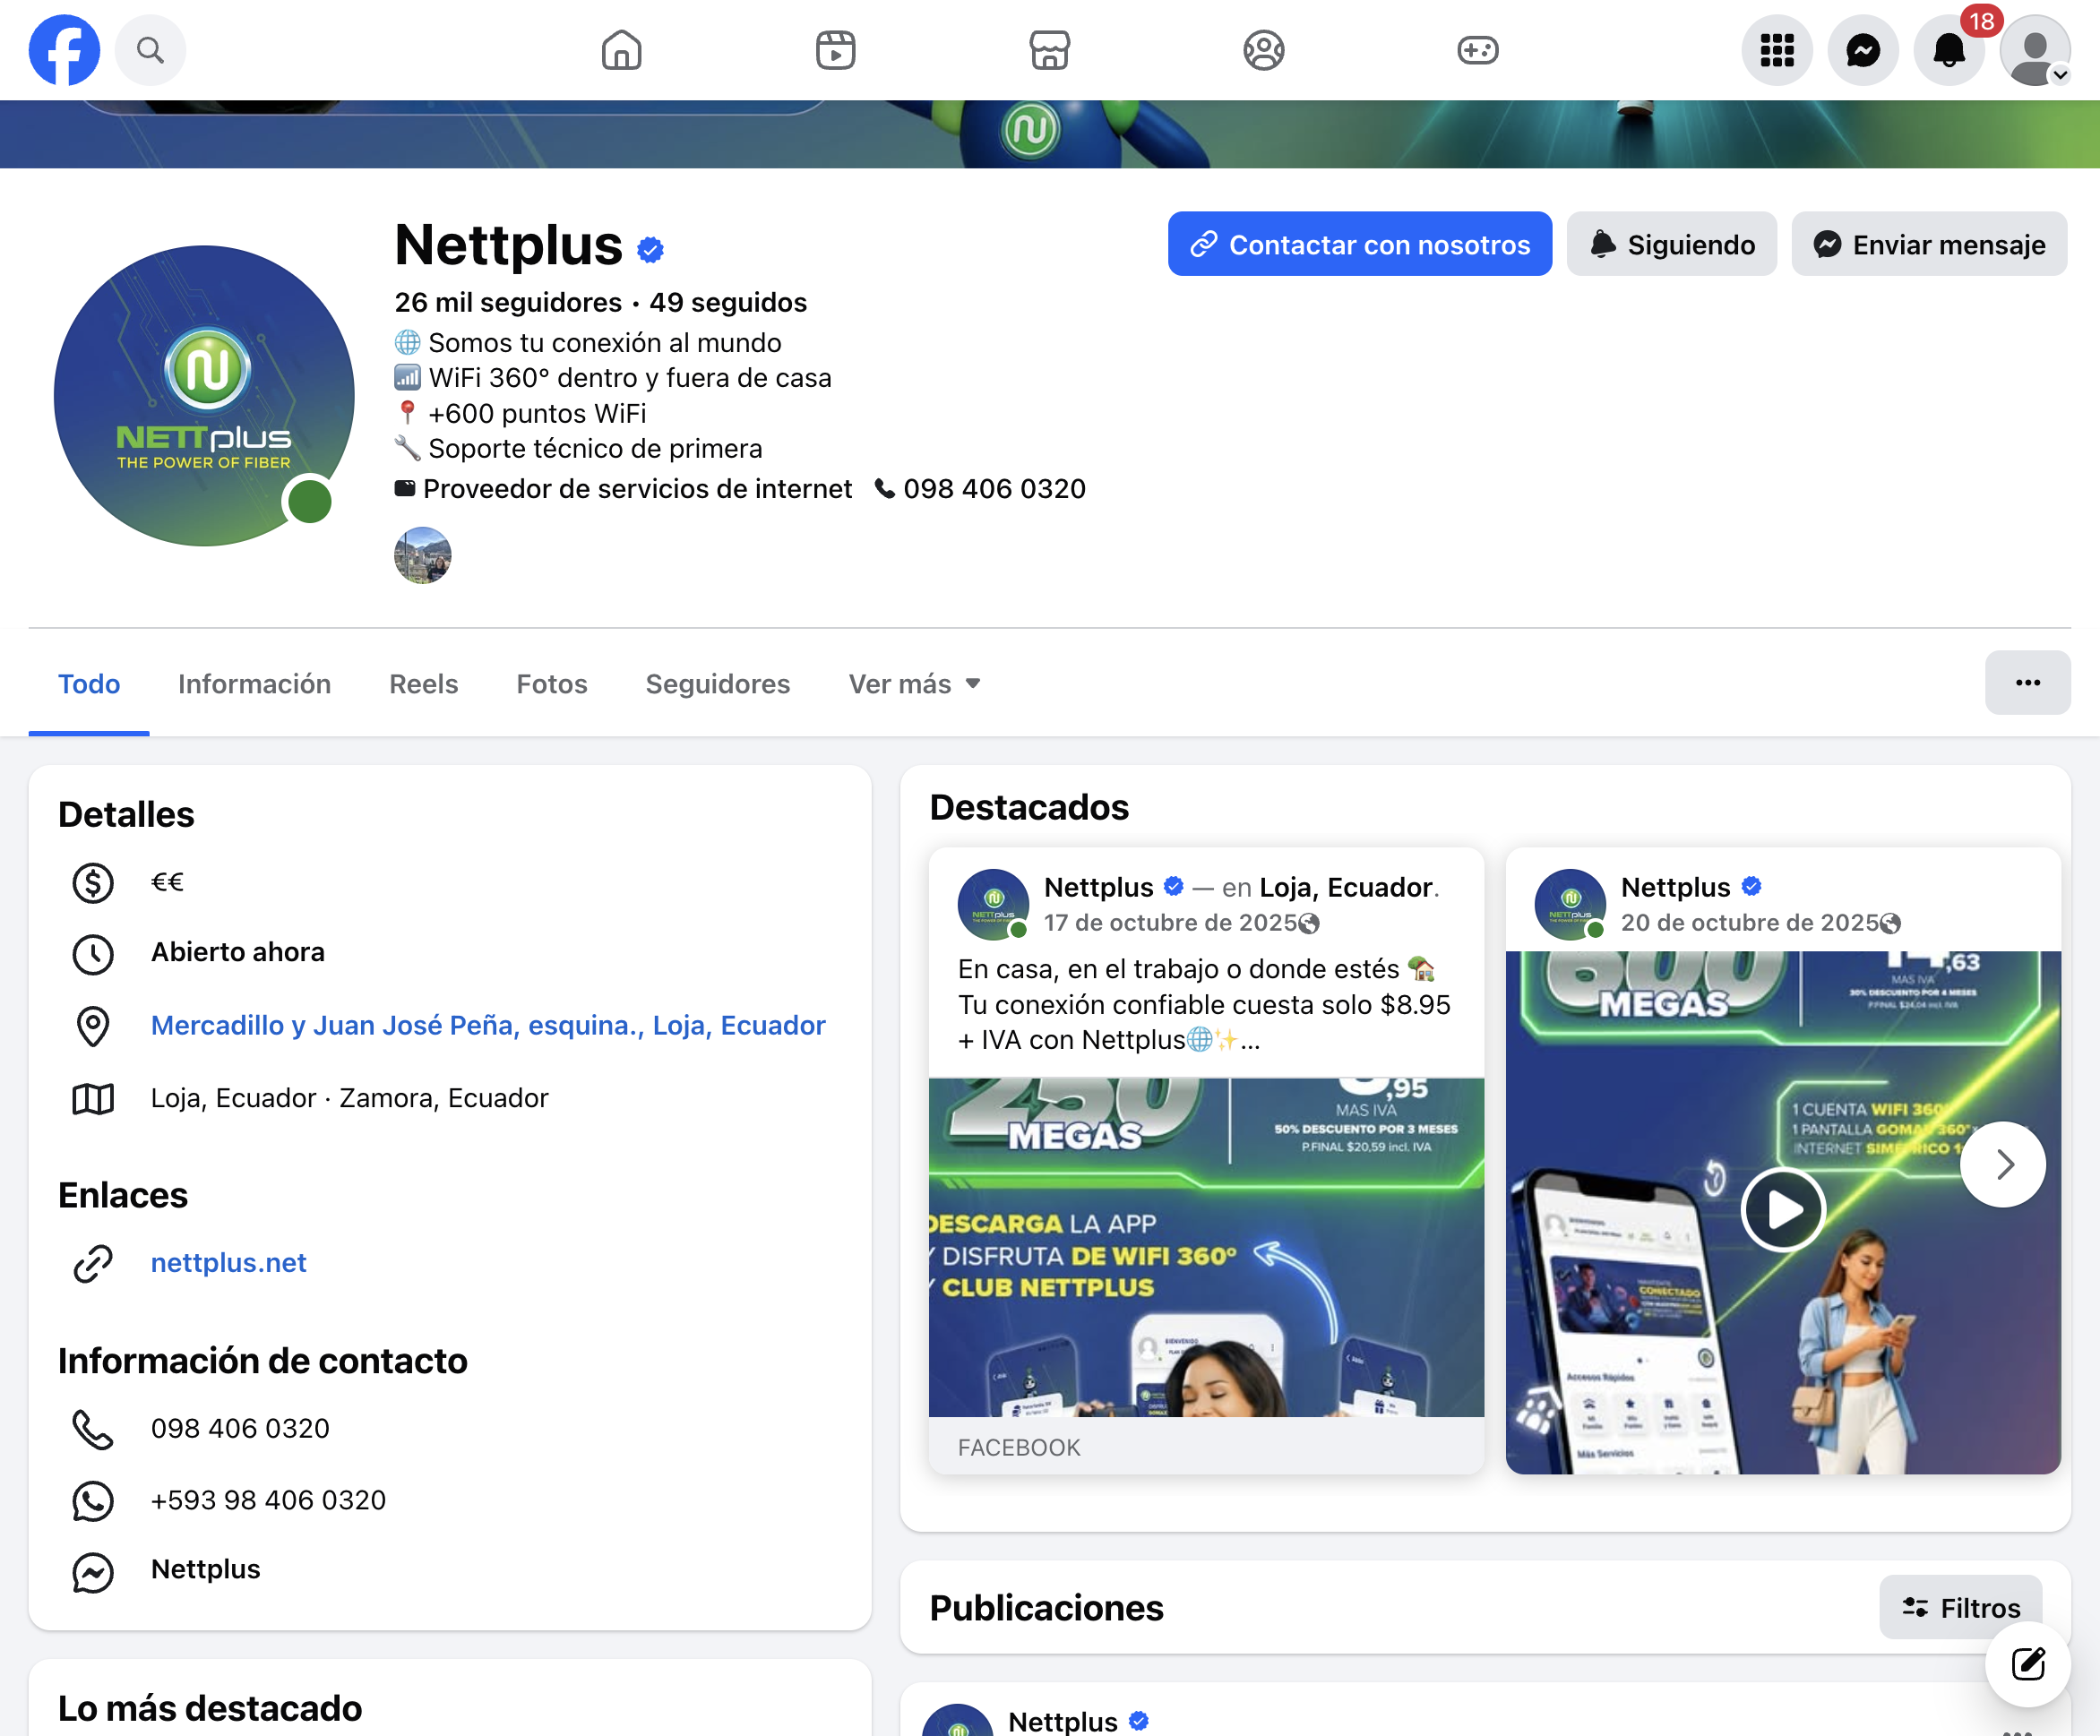
\includegraphics[width=\linewidth]{fig-fb-netplus-20260505-v2.png}
  \caption{Facebook NETPLUS con publicaciones recientes comerciales. Fuente: \url{https://www.facebook.com/Nettplusinternet}.}
\end{figure}

\begin{figure}[h]
  \centering
  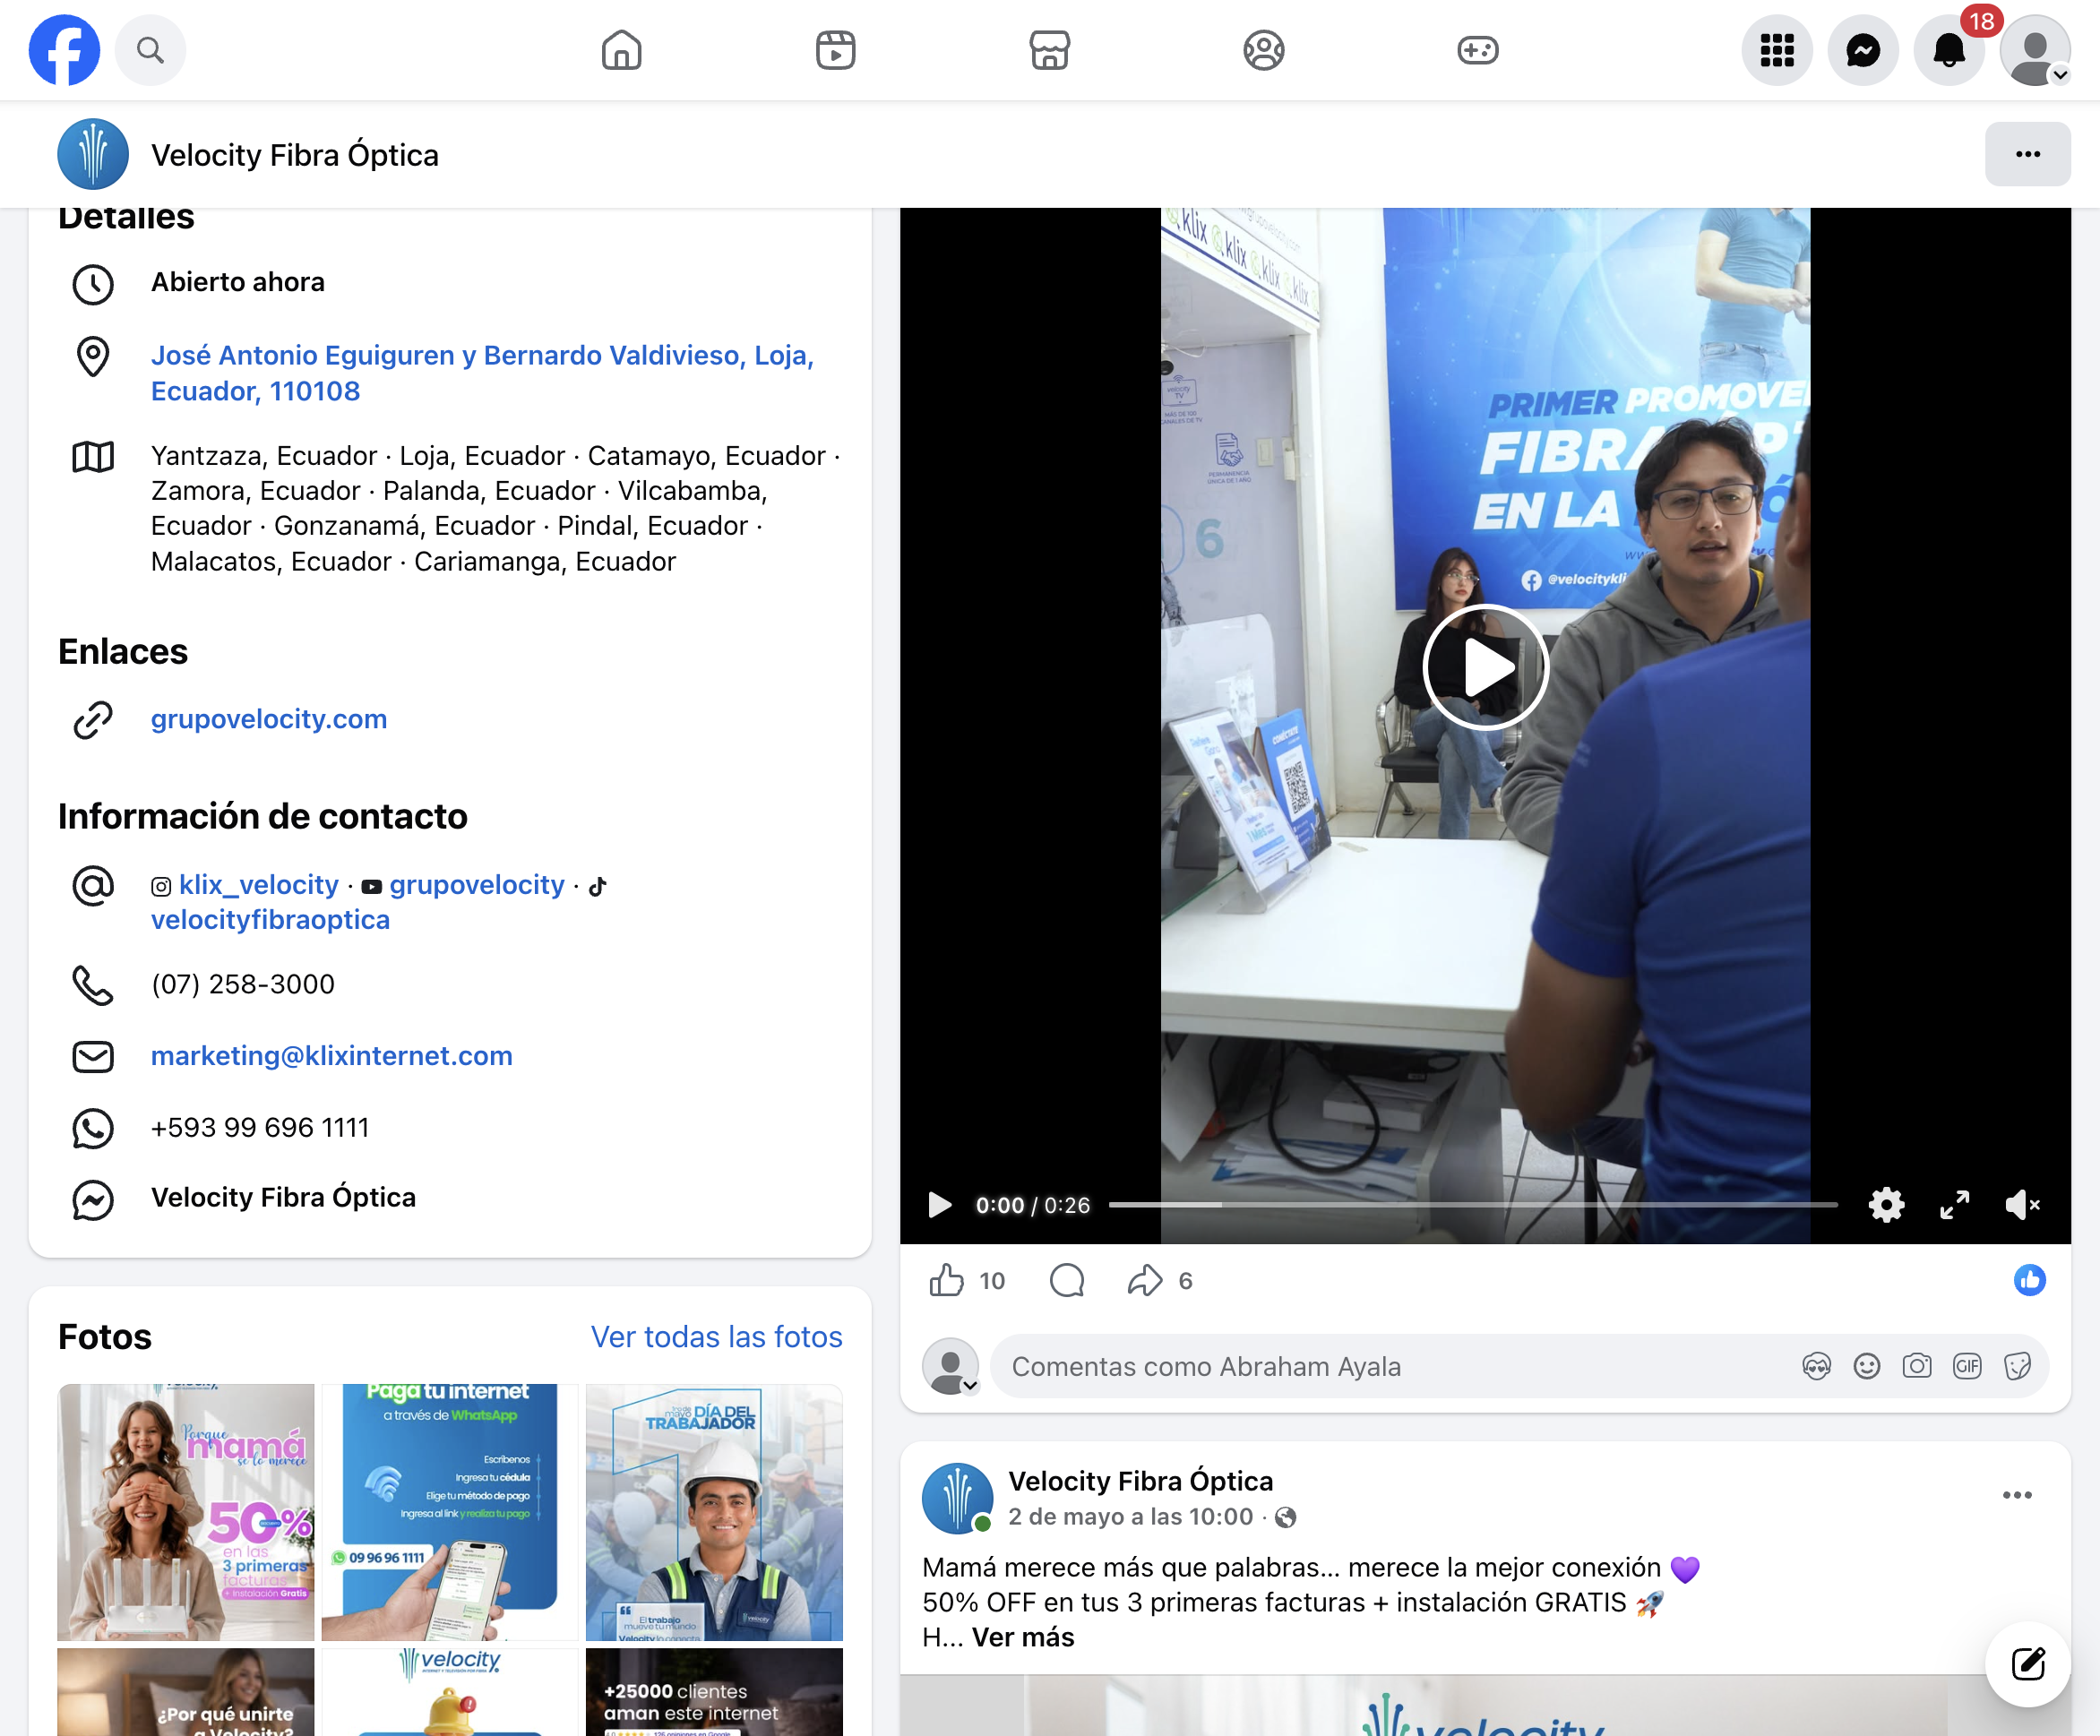
\includegraphics[width=\linewidth]{fig-fb-velocity-posts-20260505-v1.png}
  \caption{Facebook Velocity (tramo visible de publicaciones). Fuente: \url{https://www.facebook.com/velocityklix/}.}
\end{figure}

\begin{figure}[h]
  \centering
  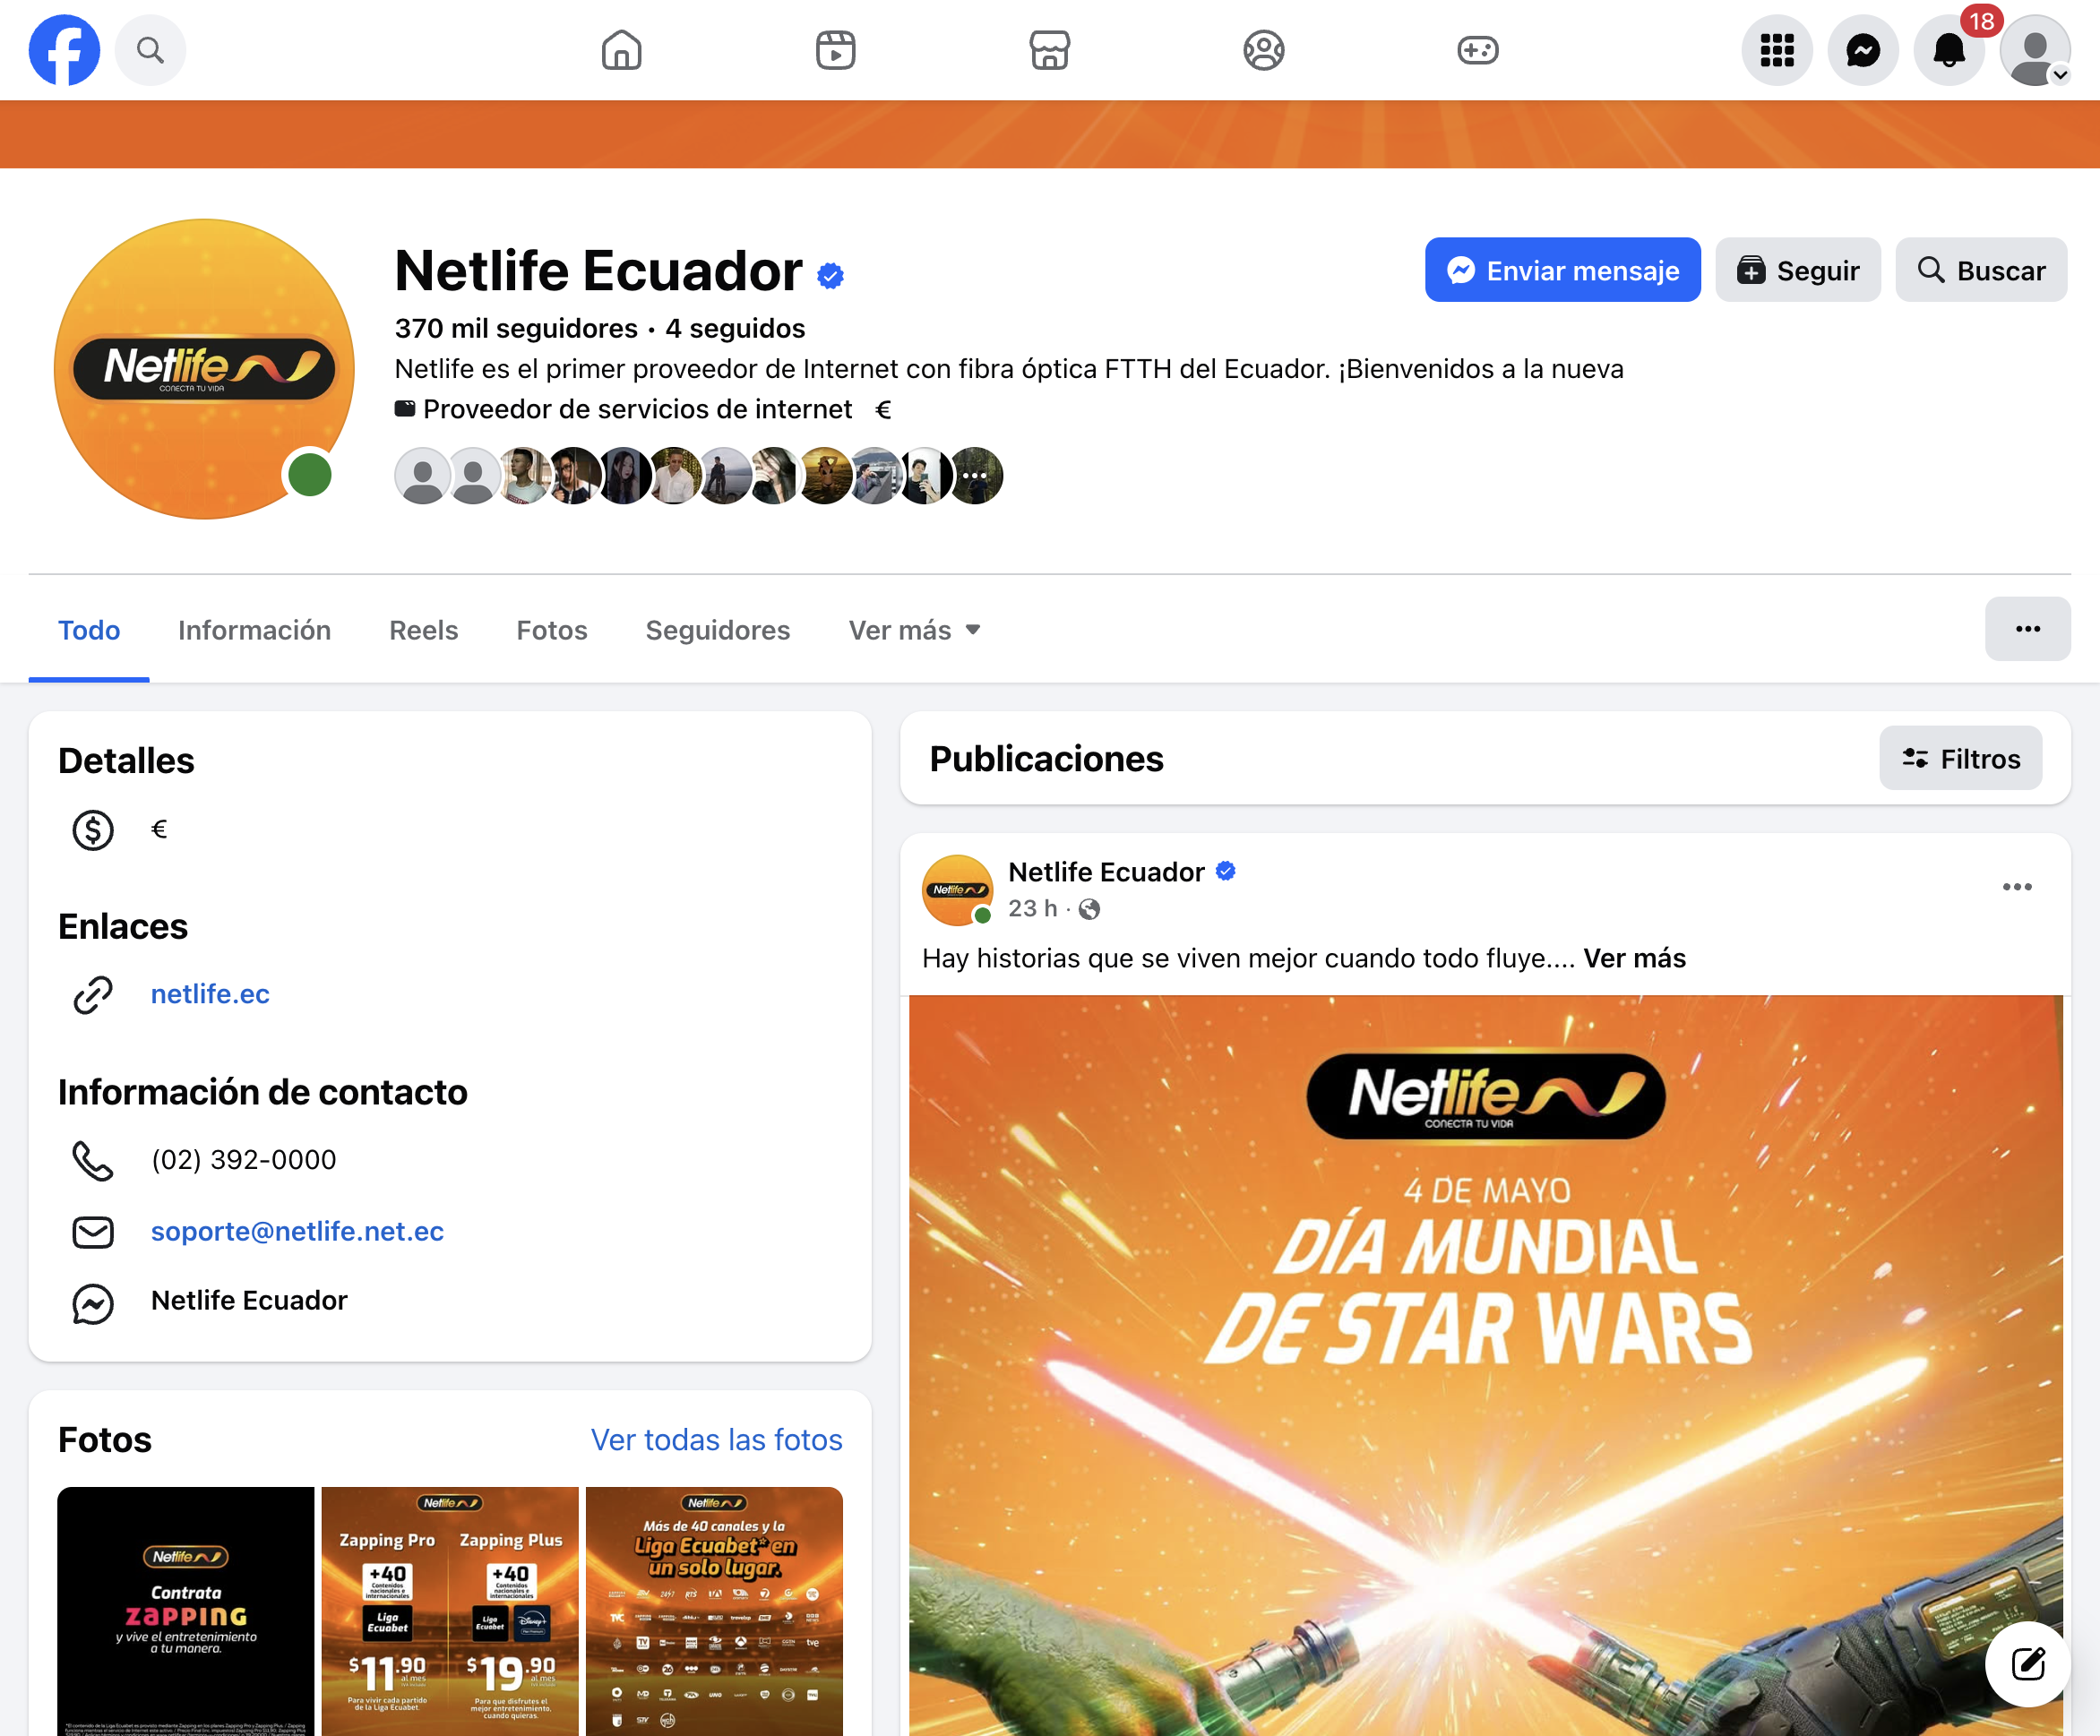
\includegraphics[width=\linewidth]{fig-fb-netlife-posts-20260505-v2.png}
  \caption{Facebook Netlife (tramo visible de publicaciones). Fuente: \url{https://www.facebook.com/netlife.ecuador}.}
\end{figure}

\begin{figure}[h]
  \centering
  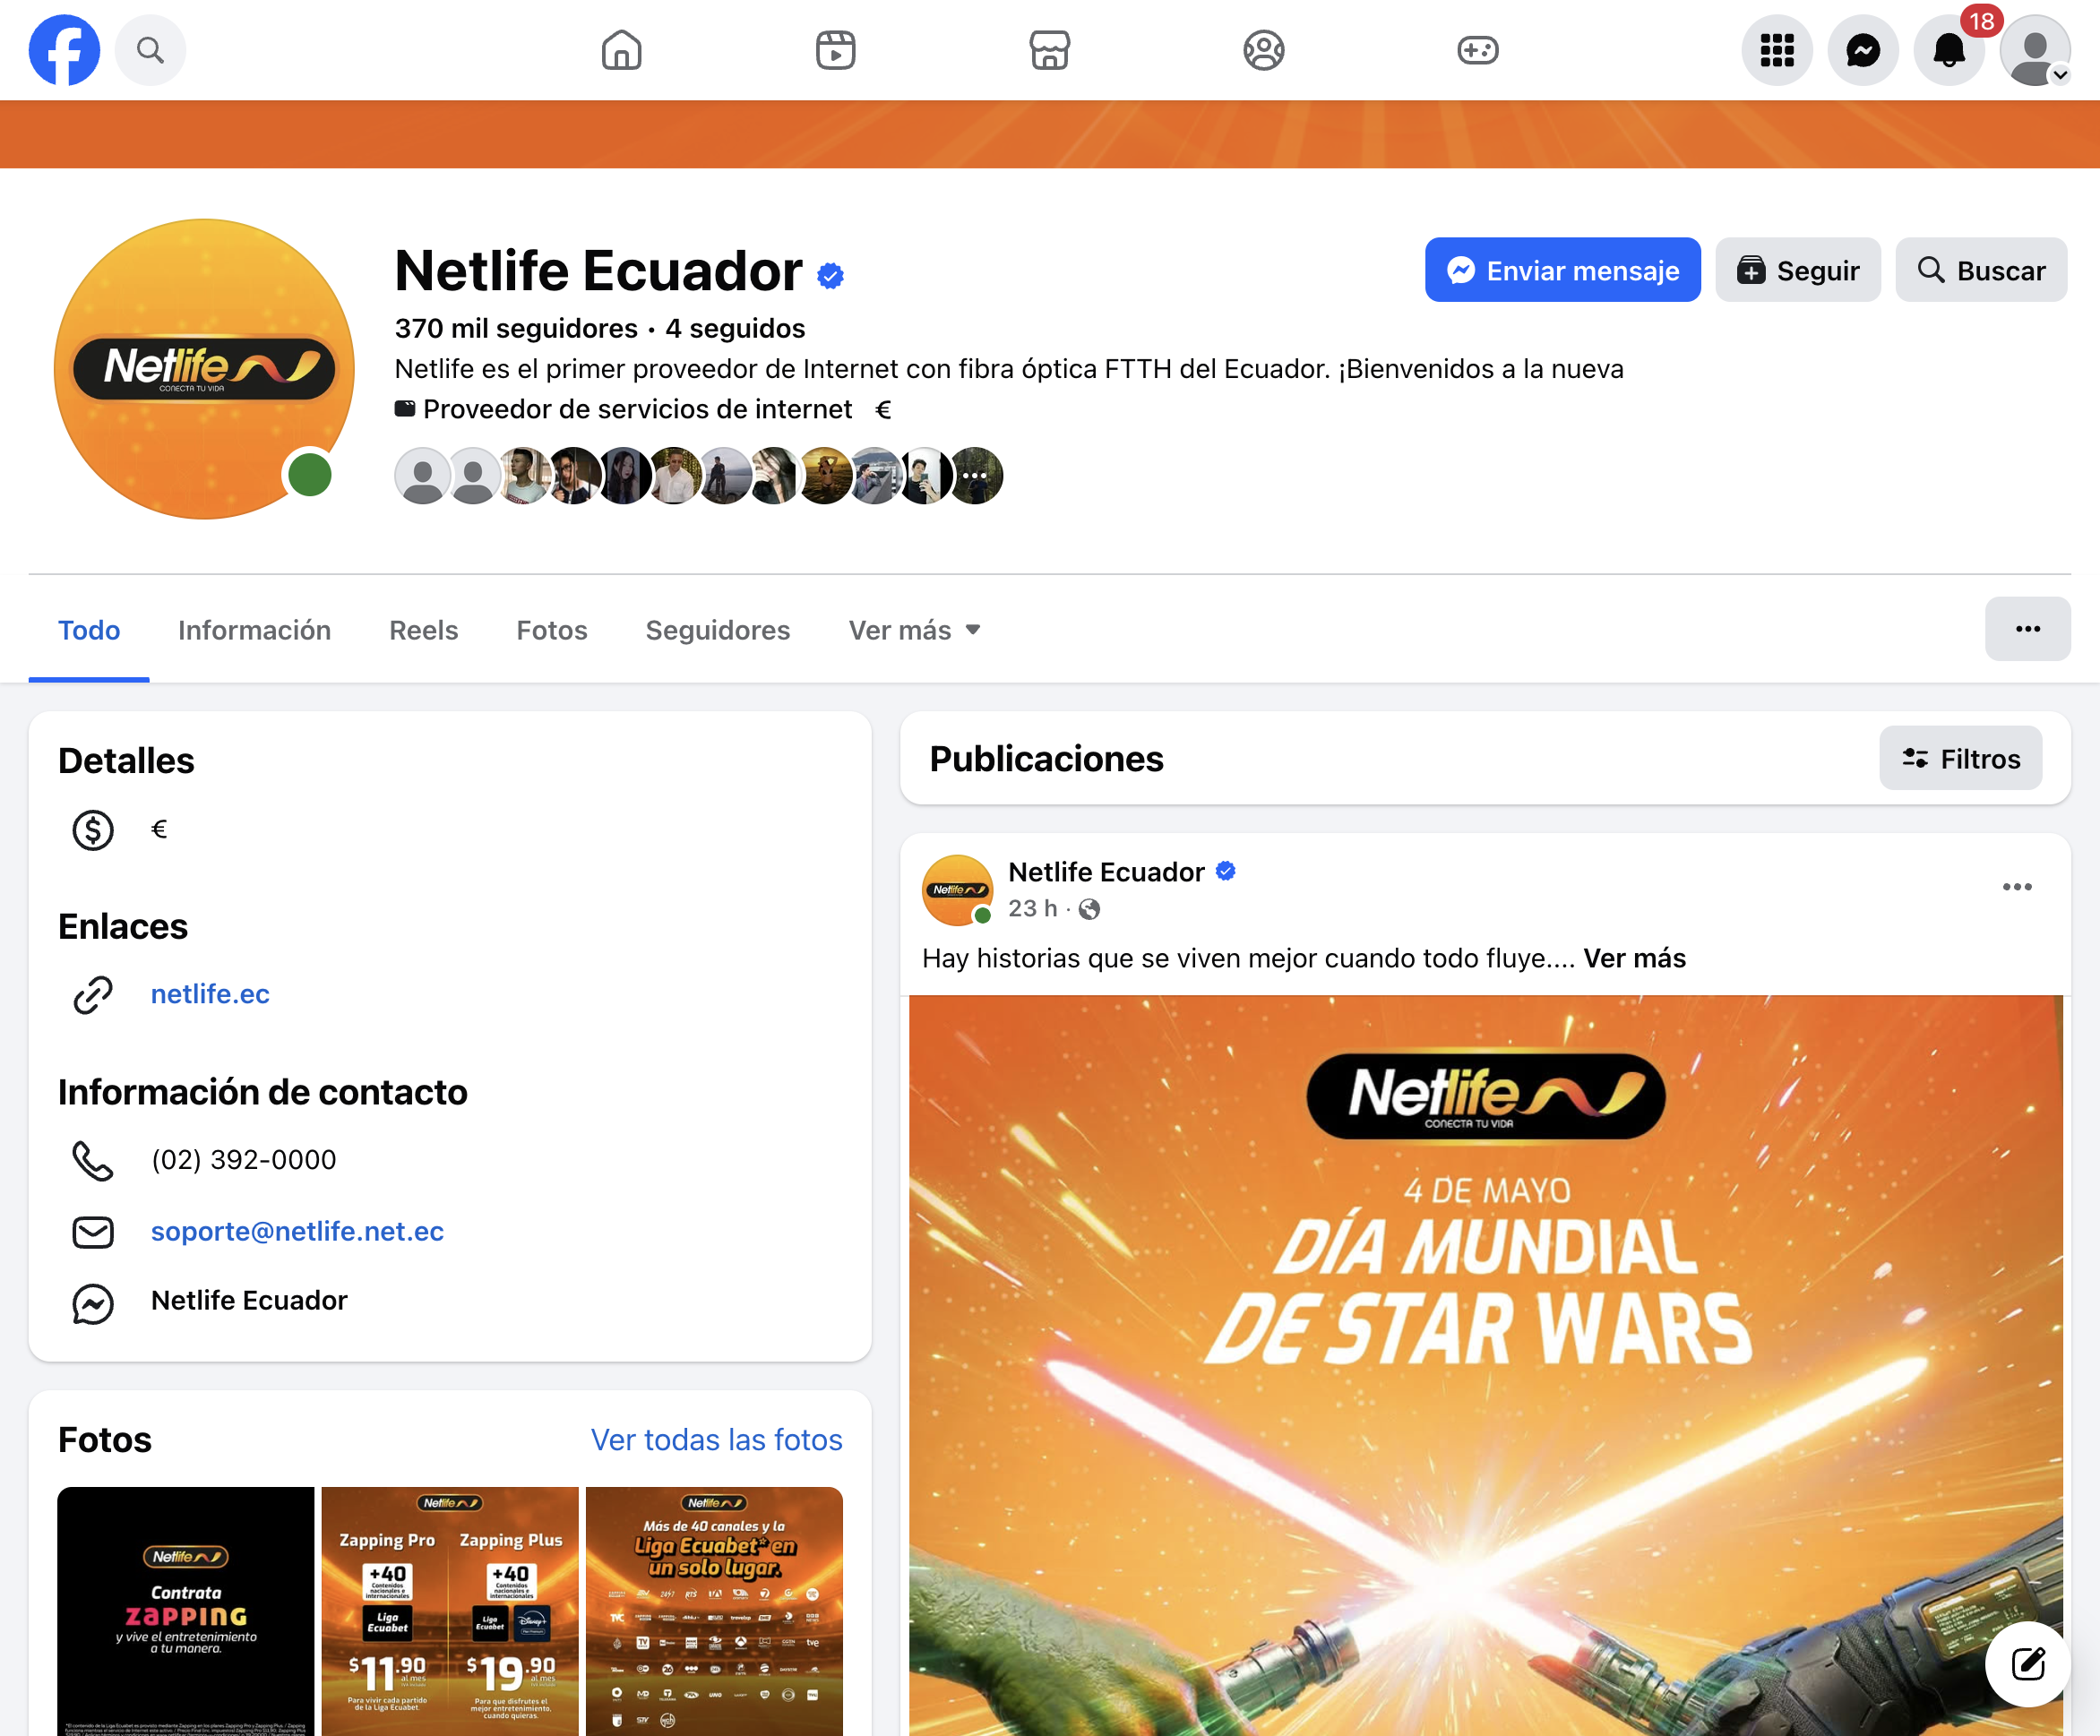
\includegraphics[width=\linewidth]{fig-fb-snel-posts-20260505-v1.png}
  \caption{Facebook SNEL (tramo visible de publicaciones). Fuente: \url{https://www.facebook.com/snel.loja}.}
\end{figure}

\begin{figure}[h]
  \centering
  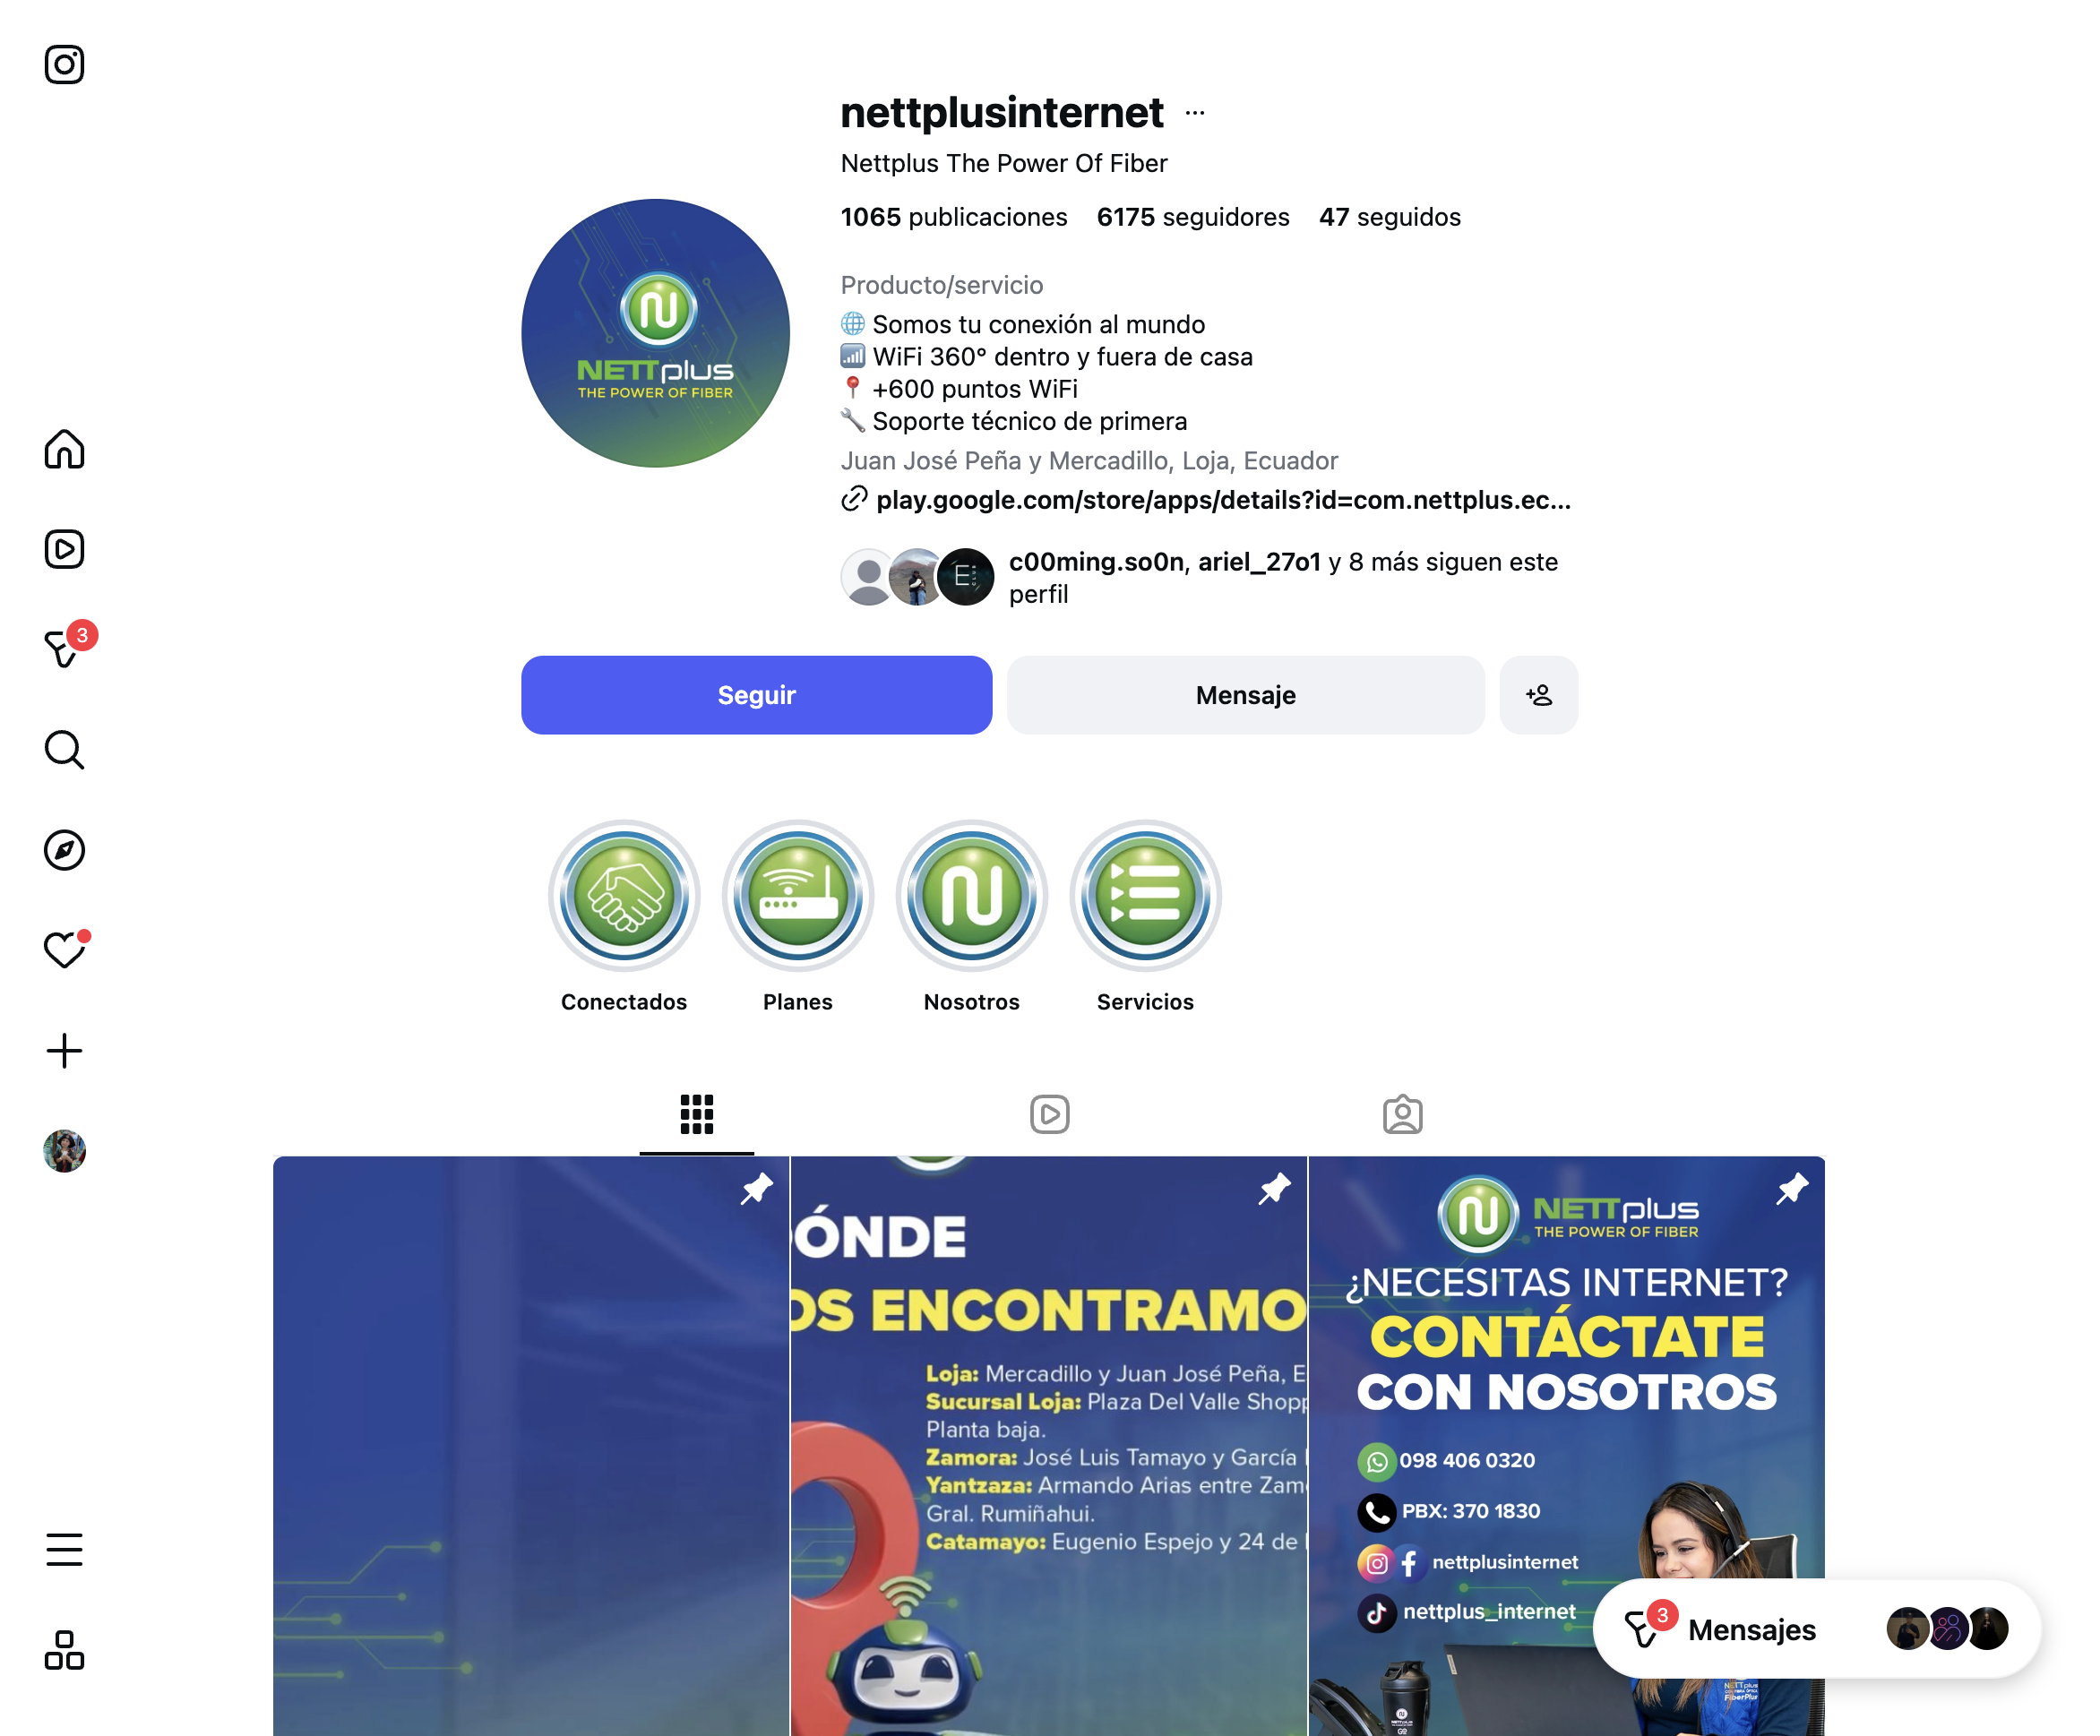
\includegraphics[width=\linewidth]{fig-ig-netplus-20260505-v1.png}
  \caption{Instagram NETPLUS oficial compartido por cliente. Fuente: \url{https://www.instagram.com/nettplusinternet/}.}
\end{figure}

\begin{figure}[h]
  \centering
  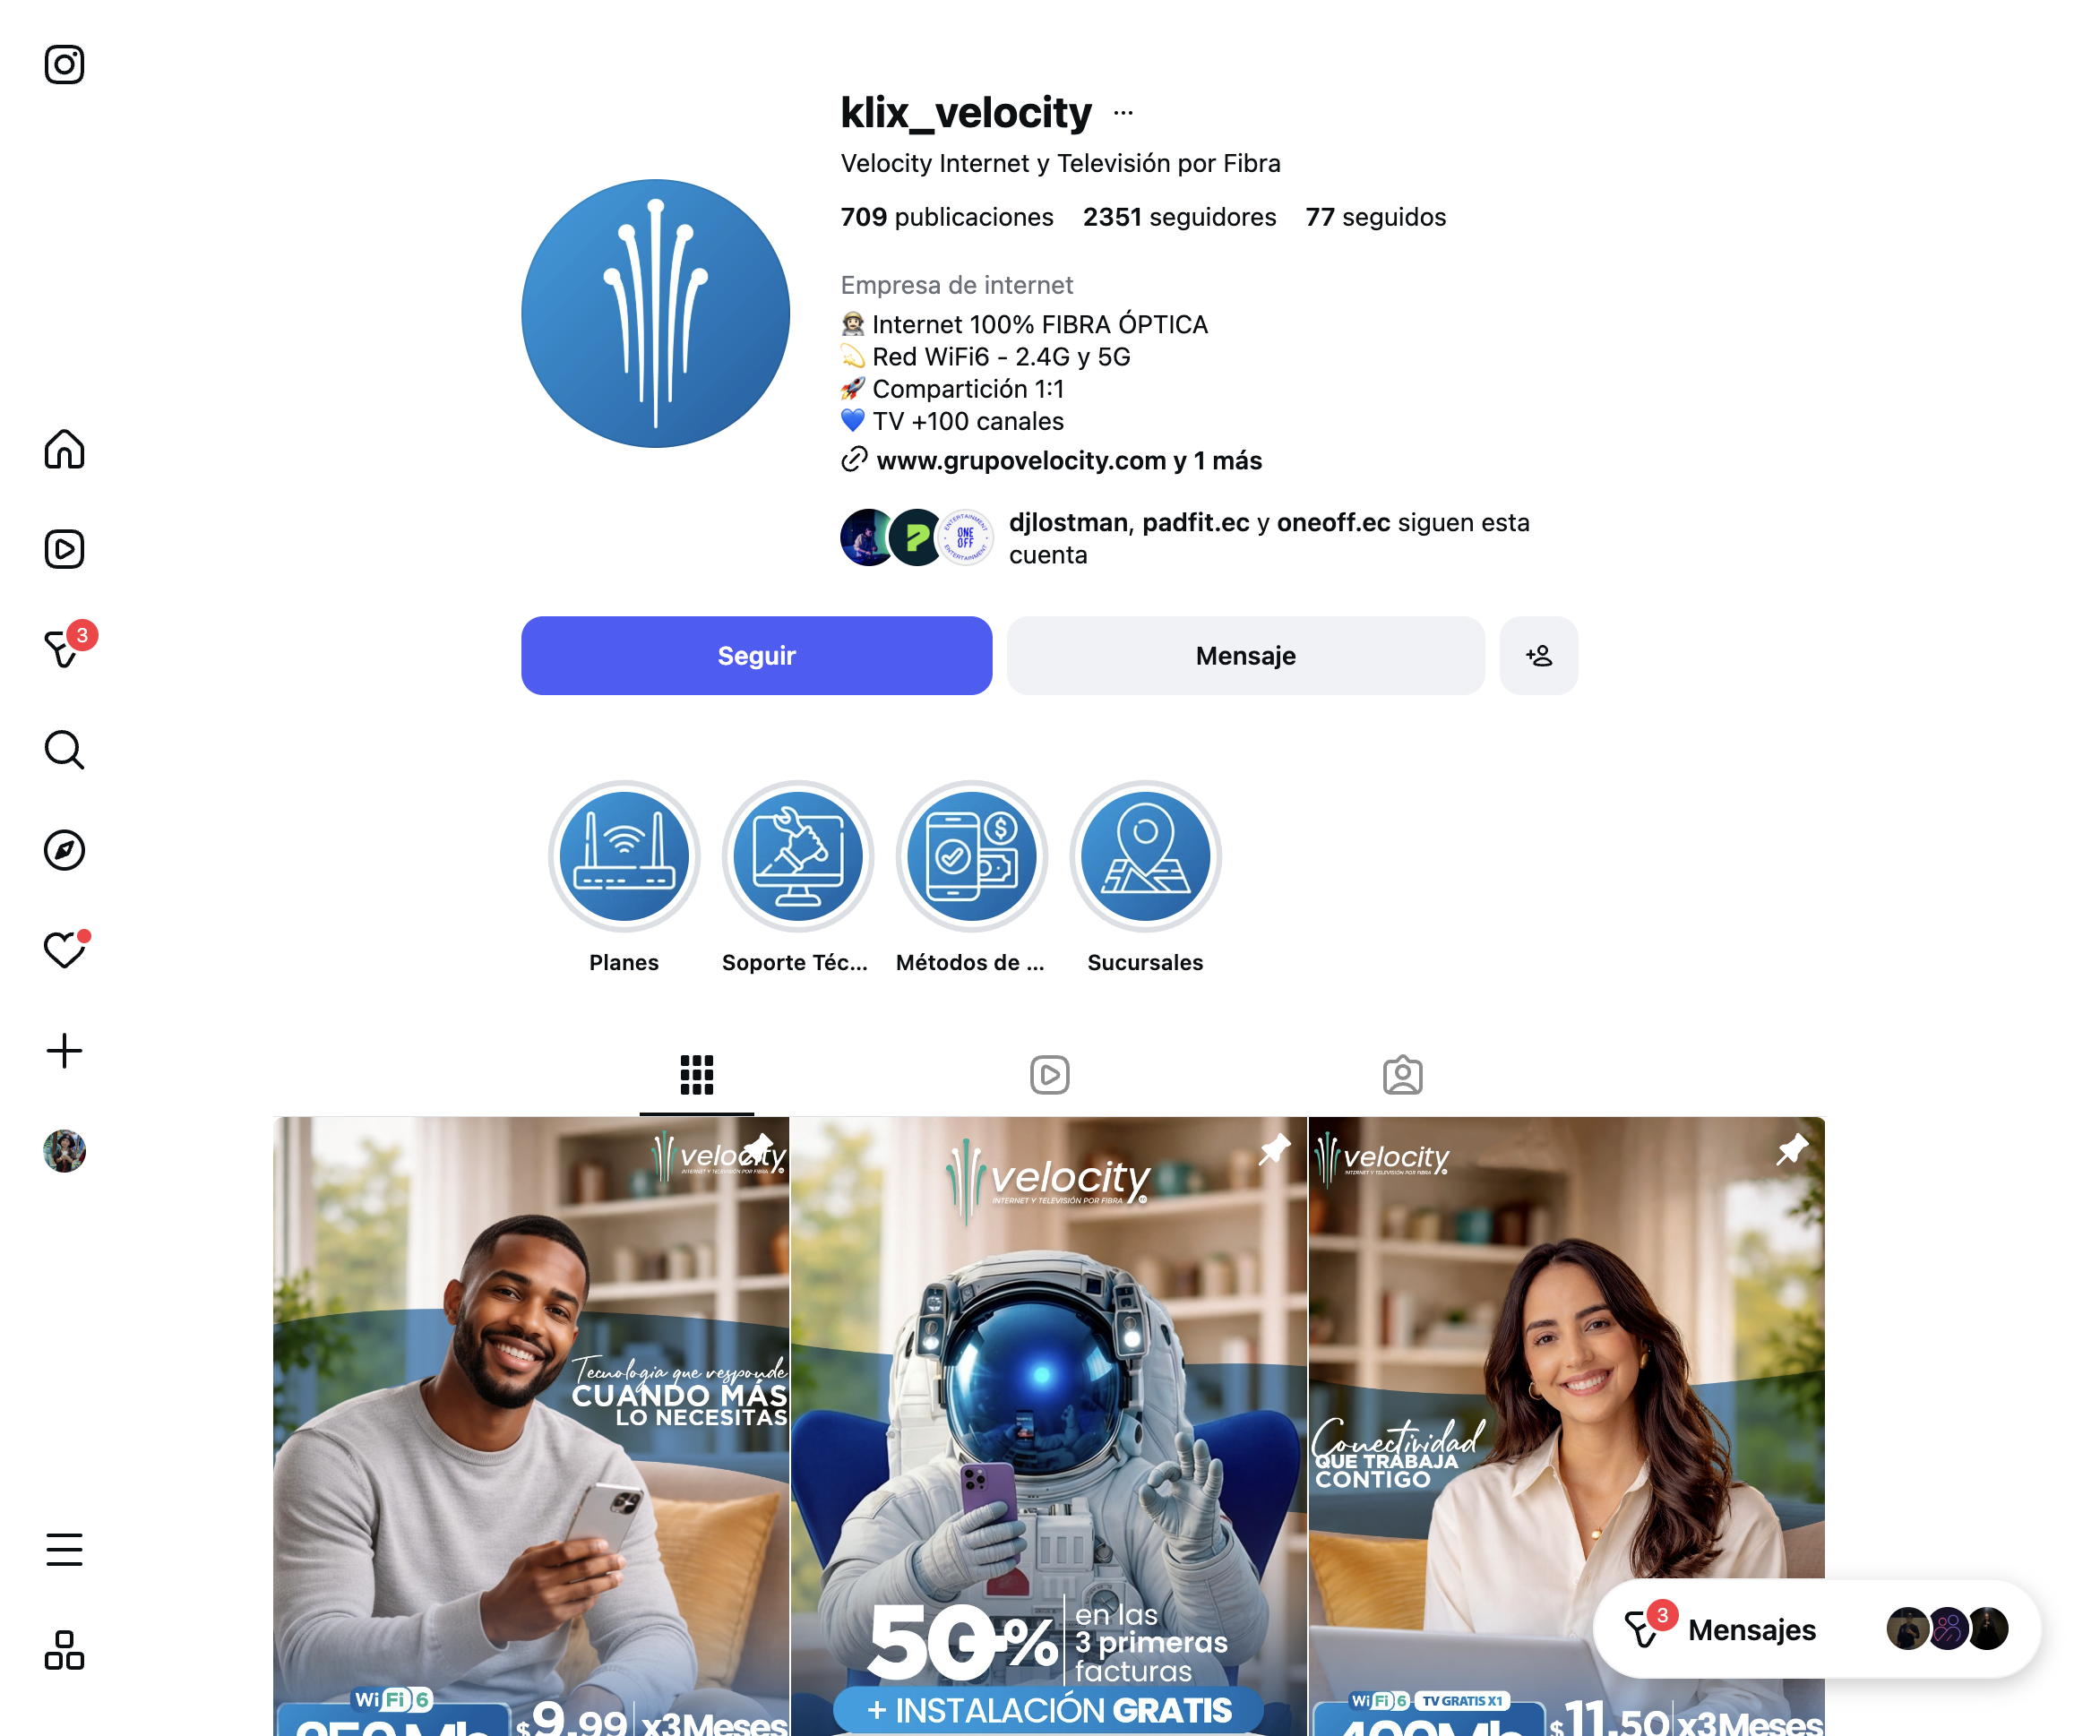
\includegraphics[width=\linewidth]{fig-ig-velocity-20260505-v1.png}
  \caption{Instagram Velocity (\texttt{@klix\_velocity}). Fuente: \url{https://www.instagram.com/klix_velocity/}.}
\end{figure}

\begin{figure}[h]
  \centering
  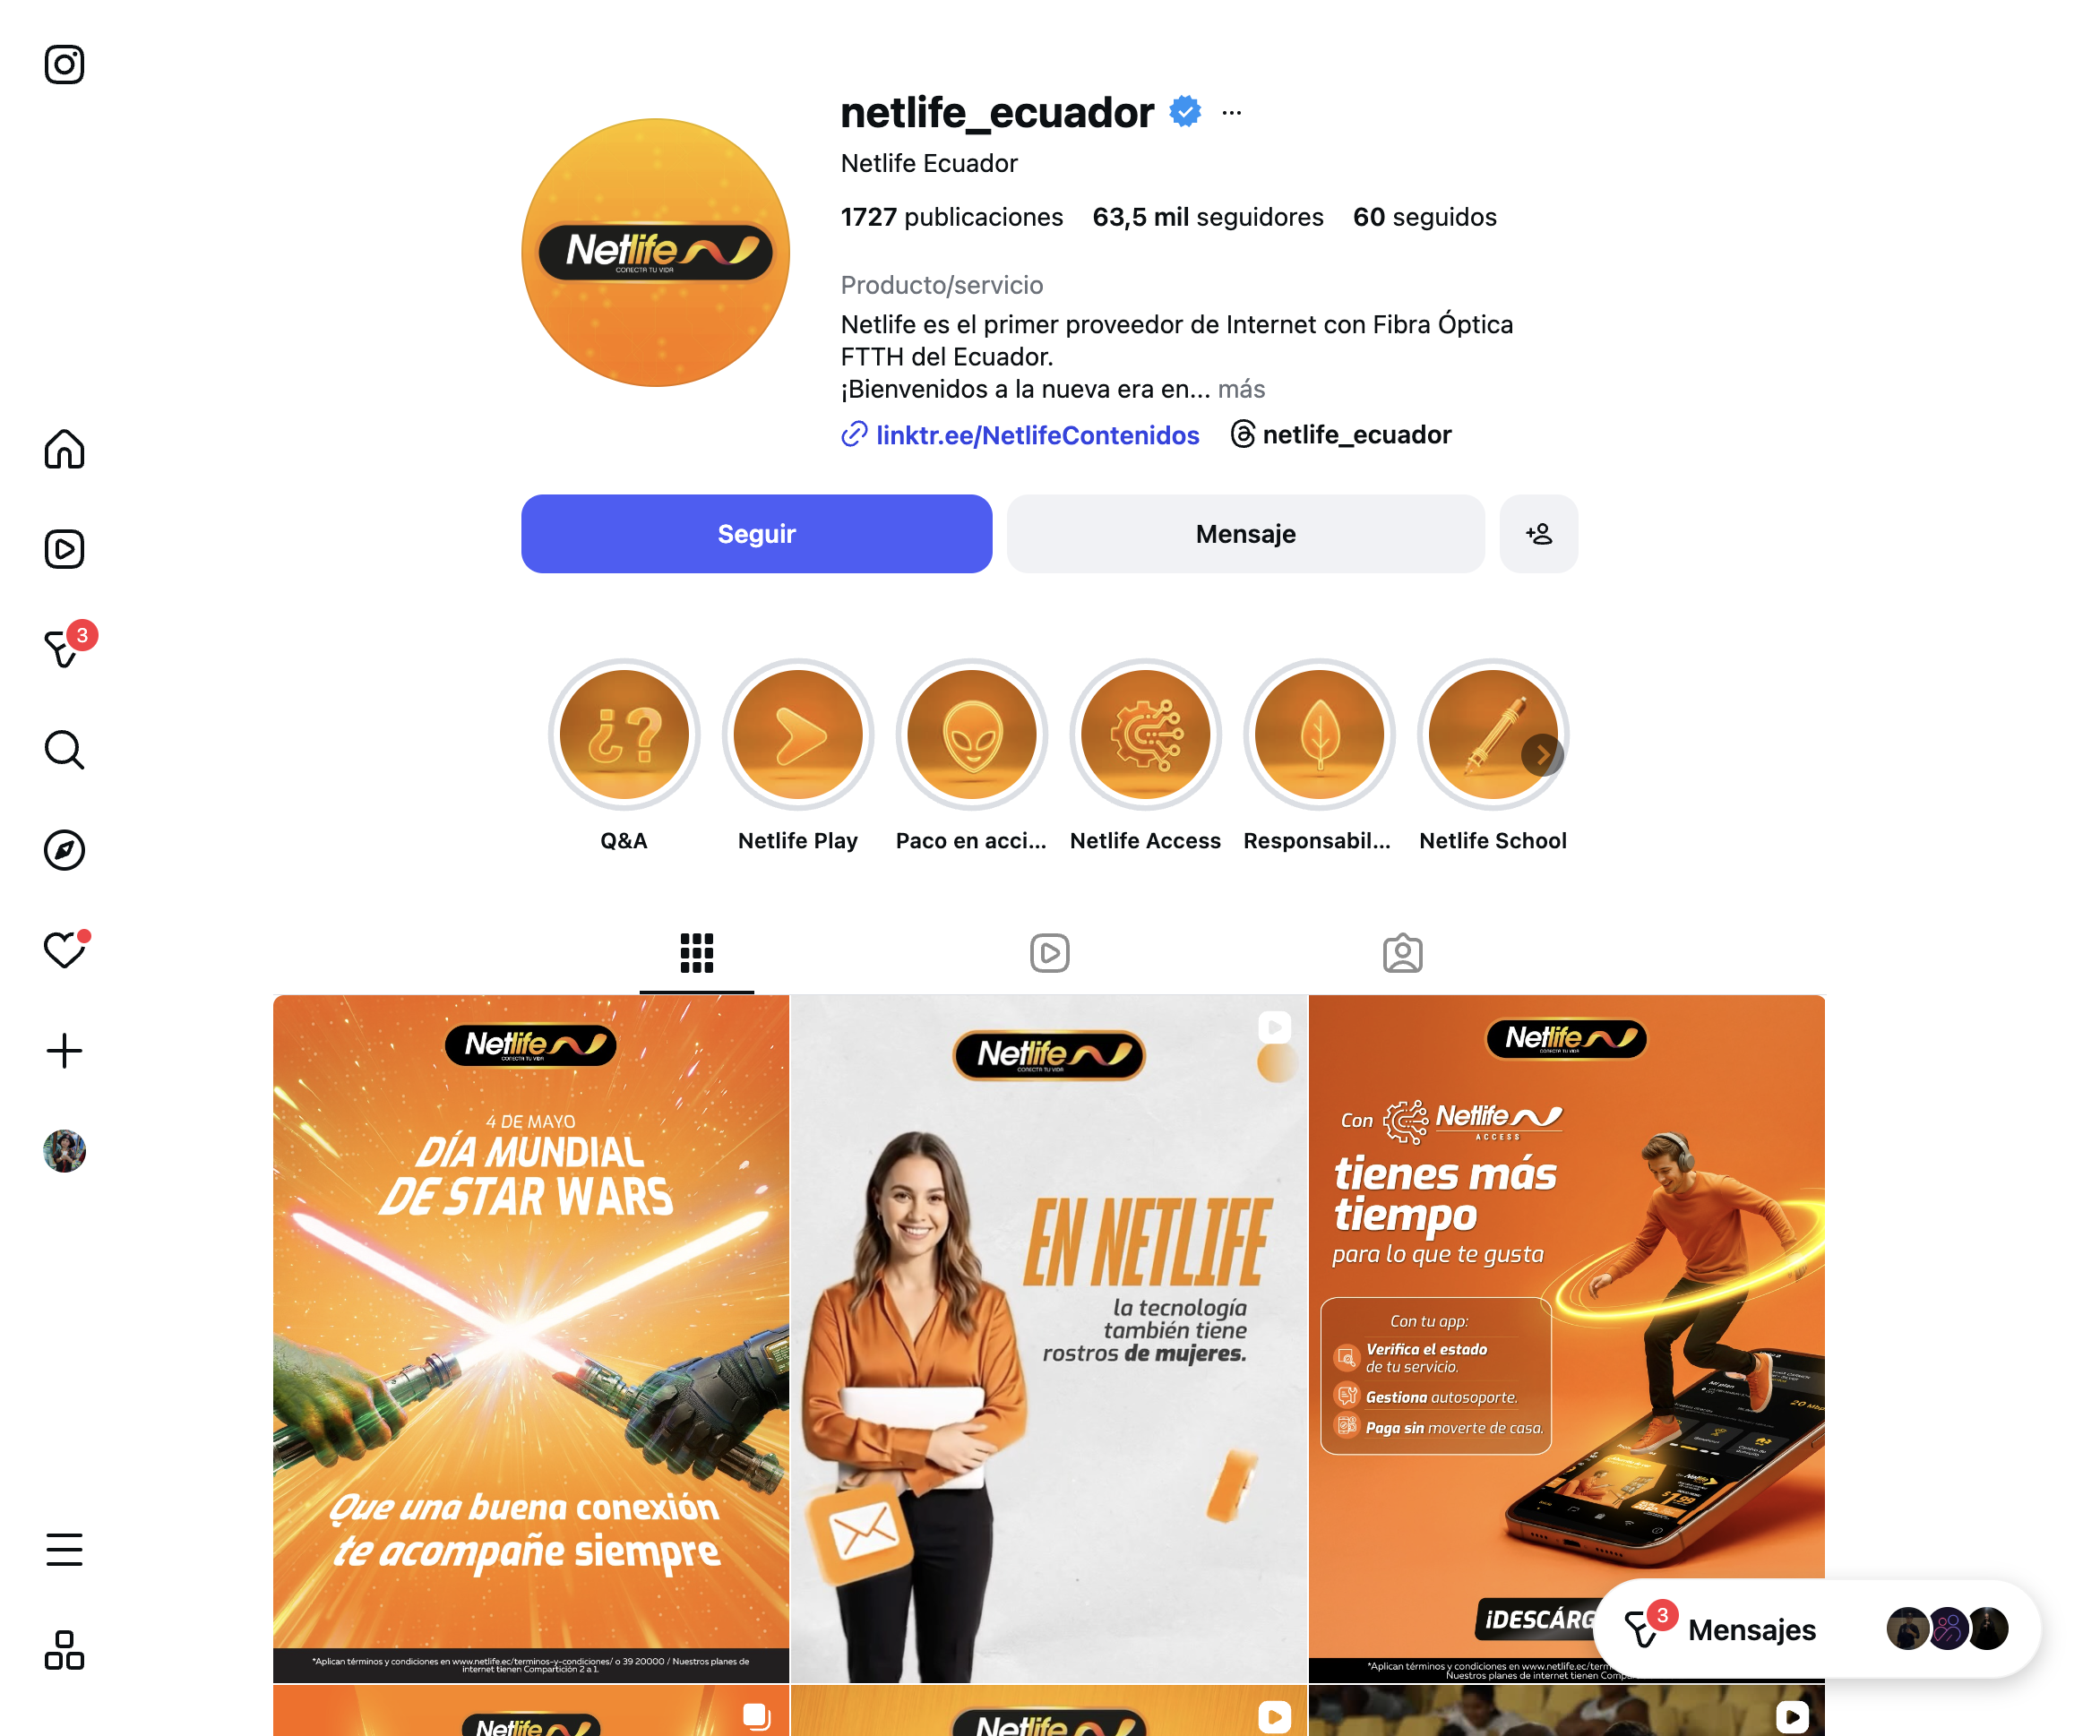
\includegraphics[width=\linewidth]{fig-ig-netlife-ecuador-20260505-v1.png}
  \caption{Instagram Netlife Ecuador. Fuente: \url{https://www.instagram.com/netlife_ecuador/}.}
\end{figure}

\section{Limitaciones}
\begin{itemize}
  \item El analisis de contenido usa una muestra visible exploratoria en una sola corrida (no historial completo de 90 dias).
  \item Algunas URLs de IG devuelven rutas no disponibles segun sesion/navegador; se uso la URL final valida compartida por cliente para Netlife.
  \item No se incluyo Meta Ads Library en esta iteracion; por tanto, ``anuncios activos'' no esta auditado de forma exhaustiva.
\end{itemize}

\end{document}
